\section{Efficiencies}
% It is nice to add here the method you use to 
% estimate the efficiency, and at least a plot of the 
% efficiency(ies) itself.

The overall efficiency is the product of the generator level efficiency ($\epsilon^{gen\&acc}$) which includes the geometrical acceptance of the detector and generator level cuts efficiency, the combined reconstruction and selection efficiency ($\epsilon^{rec\&sel}$) and the trigger efficiency ($\epsilon^{trig}$). For first approach we are using $\epsilon^{full} = \epsilon^{rec\&sel} \times \epsilon^{trig}$.


\subsection{Acceptance efficiency}
Obtained individual generator level efficiencies for signal and normalization channels is presented in the table below:


\vspace*{0.5cm}
\mbox{~}
\begin{tabular}{|l|l|c|c|}
\hline
Year & Magnet & $B_{u} \to J/\psi KK\pi$ & $B_{u} \to \psi' K$ \\
\hline
2011 & Up   & $0.15678 \pm 0.00041$ & $0.15311 \pm 0.00039$ \\
2011 & Down & $0.15713 \pm 0.00039$ & $0.15390 \pm 0.00039$ \\
2012 & Up   & $0.16175 \pm 0.00060$ & $0.1559  \pm 0.000393$ \\
2012 & Down & $0.1609  \pm 0.0013$  & $0.1562  \pm 0.000391$ \\
\hline
\end{tabular}
\vspace*{0.5cm}

The average of four ratios is $\epsilon_{gen\&acc}^{KK\pi} / \epsilon_{gen\&acc}^{\psi'K} = 1.028 \pm 0.003$ is chosen as the resulting ratio of geometrical acceptance efficiencies (uncertainty is statistical only). The maximal devistion from the average is taken as systematic uncertainty and equals $1\%$.

\subsection{Full efficiency}

For the signal channel we have $N_{MC-input}^{KK\pi} = 1538248$ events. Number of events was obtained from get-bookkeeping-info and by grepping Ganga's output. On whole all generated events we apply reconstruction, WG selection and custom selection criteria with trigger cuts and MC-true included. After applying all selection criteria we get distribution on Figure ~\ref{fig:mc-signal}, which is fitted by Double-Sided Crystal Ball function with all parameters set to be free. We get $N_{mc-sig} = 22394 \pm 149$ events. Now we can calculate 
$$\epsilon^{full}_{sig} =  \frac { N_{mc-sig} }{ N_{MC-input}^{KK\pi} } =  (1.46 \pm 0.01) \times 10^{-2}$$

Same procedure for normalization channel. Here we have $N_{MC-input}^{\psi'K} = 3673304$ events. Fit is on Figure ~\ref{fig:mc-norm}, from it we get $N_{mc-norm} = 32775 \pm 183$. And the efficiency is 
$$\epsilon^{full}_{norm} =  \frac { N_{mc-norm} }{ N_{MC-input}^{\psi'K} } =  (0.892 \pm 0.005) \times 10^{-2}$$


\pagebreak
\subsection{Braching ratio}

Now we can obtain braching ratio:

$$
\frac{\mathcal{B}(B_{u} \to J/\psi \, KK\pi)}{\mathcal{B}(B_{u} \to (\psi(2S) \to J/\psi \pi\pi) \, K)} = \
\frac{ N_{sig.} }{ N_{norm.} } \times \frac{\epsilon_{gen\&acc}^{KK\pi} }{ \epsilon_{gen\&acc}^{\psi'K}} \times \frac{\epsilon_{sig.}^{full}}{\epsilon_{norm.}^{full}} =
$$
$$
= \frac{224 \pm 26}{9153 \pm 68} \times (1.028 \pm 0.003) \times \frac{(1.46 \pm 0.01) \times 10^{-2}}{(0.892 \pm 0.005) \times 10^{-2}} = \
0.041 \pm 0.005 = \mathcal{R}
$$

With ratio $\mathcal{R}$ we can now obtain: 
$$
\mathcal{B}(B_{u} \to J/\psi \, KK\pi) = \mathcal{B}(B_{u} \to \psi(2S) K) \times \mathcal{B}(\psi(2S) \to J/\psi \pi\pi) \times \mathcal{R} \simeq
$$

$$
\simeq 6.27 \times 10^{-4} \times 0.34 \times \mathcal{R} = (8 \pm 1) \times 10^{-6}
$$


\begin{figure}[here]
\centering
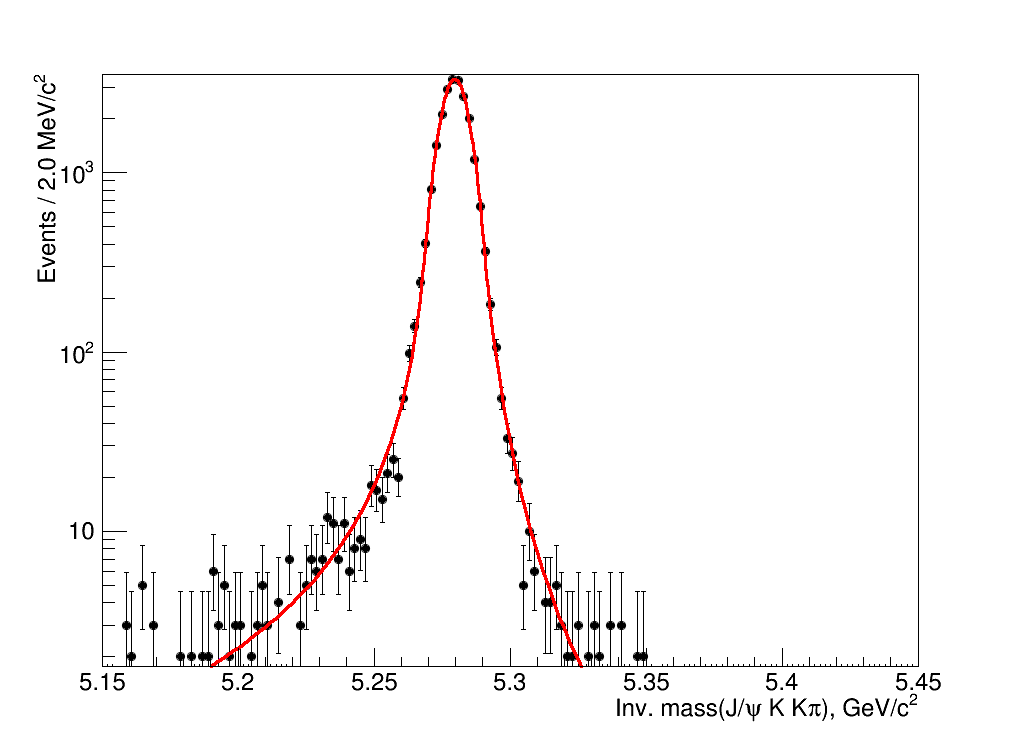
\includegraphics[width = 0.8\textwidth]{img/MC-signal.png}
\caption{Signal MC distribution with all cuts applied}
\label{fig:mc-signal}
\end{figure}


\begin{figure}[here]
\centering
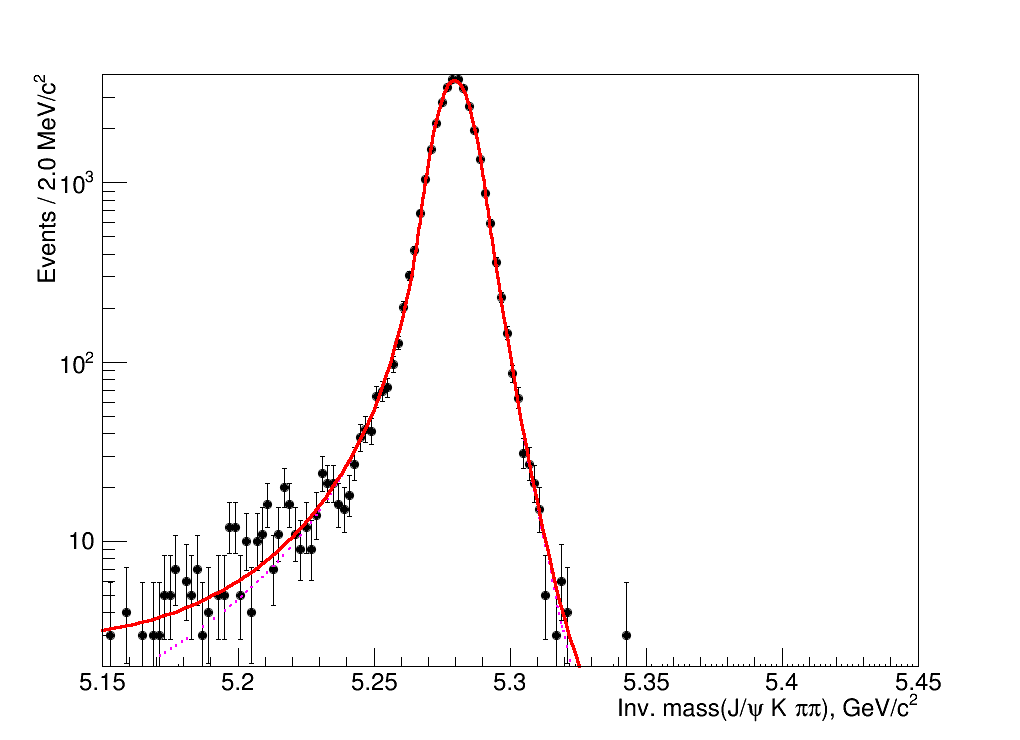
\includegraphics[width = 0.8\textwidth]{img/MC-norm.png}
\caption{Normalization channel MC distribution with all cuts applied}
\label{fig:mc-norm}
\end{figure}


